\section{Requirements} \label{sec:Requirements}
A system could be summarised roughly as a solution to one or more problems. One
of the first steps in order to build this kind of solution is to try to
understand the problem -- that is, try to map the requirements of the software. 

The definitions of functional and non-functional requirements from Appendix 1
(\ref{appendix1}) will be employed when trying to classify the requirements and
model the problem domain. The initial iterations will be focused more on the
functional and usability requirements, paying some attention as well to
specific non-functional requirements such as performance and security.

Any personal accounting system should be able to provide accurate and relevant
summaries of an individual's financial status. In order to do this, the user
needs to be able to supply the system with the necessary data, so that it can
be analysed and properly converted into knowledge.

It seems fair to infer that nowadays most of a user's financial transactions
happen in ways that can be listed electronically (usually via their bank or
credit card statements) -- a study by Payments UK
(\citeyear{paymentsUK2017summary}), for example, indicates that there has been
a rise in debit card payments over the past few years, and that the volumes of
this type of transaction is likely to be higher than that of cash payments by
the year 2021. Therefore, an assumption has been made that the users will
require means of uploading a list of their financial transactions into the
system.

The system created for this project intends to do just this. Its main feature,
however, will be to allow the user to categorise expenditure based on patterns
in the entries' descriptions. There must also be a feature to allow the user to
view summaries of the income and expenditure over a period of time, as well as
one to forecast budgets for future periods based on the ``financial behaviour''
analysed.

\subsection{Functional Requirements} \label{sec:Requirements.FunctionalRequirements}

Use case diagrams are UML constructs which were developed by Jacobson et al.
(1992, cited \cite[][p.~154]{bennett2010object}). The use case diagram on
Figure \ref{fig:UseCaseDiagram} is used to illustrate the functional
requirements identified for this project:
\begin{figure}[ht!]
  \begin{center}
    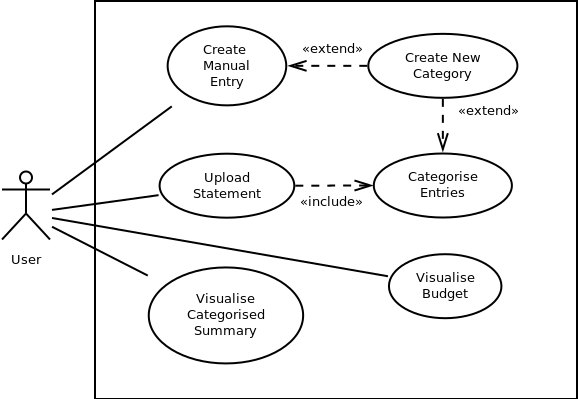
\includegraphics[width=14cm]{./contents/img/Use_Case_Diagram.png}
  \end{center}
  \caption{Use Case Diagram}
  \label{fig:UseCaseDiagram}
\end{figure}
\FloatBarrier

Table \ref{tab:UseCaseDescriptions} lists the descriptions for the use cases
listed above. The first iteration had them all in a single table, but at
subsequent ones more details were identified
\begin{table}[ht!]
  \centering
  \begin{tabular}{|p{4cm}|p{12cm}|}
    \hline
    \textbf{Use Case}&\textbf{Description}\\
    \hline
    Upload Statement&The user must be able to upload a list of their
                     financial transactions, most likely their bank
                     or credit card statements, in a valid format, and all
                     entries should be categorised based on specific patterns\\
                    &\emph{Includes}: Categorise Entries\\
    \hline
    Create Manual Entry&The user should be able to create a manual entry for
                        income or expenditure, include a date, amount and
                        description, and either choose an existing category for
                        it or create a new one in the process\\
                       &\emph{Extends}: Create Category\\
    \hline
    Visualise Categorised Summary&The use must be able to visualise
                                  a summary of their income and expenditure
                                  over a period of time\\
    \hline
    Visualise Budget&The user must be able to visualise a budget for future
                     periods based on their income and expenditure data 
                     already entered\\
    \hline
    Categorise Items&Analyse the current entry and assign it to a category\\
                    &\emph{Extends}: Create Category\\
    \hline
    Create Category&Creates a new category with the name suggested by the
                        user\\
    \hline
  \end{tabular}
  \caption{Use Case Descriptions} \label{tab:UseCaseDescriptions}
\end{table}
\FloatBarrier

The wireframe below (Figure \ref{fig:Wireframe.CreateManualEntry}) was created
to better illustrate the \emph{Manual Entry} requirement from the point of view
of the user. It shows an example of an entry for a laptop and a licence for a
proprietary operating system, which can then be broken down among different
categories. The user has the option to use the percentage or the amount boxes
in order to provide a breakdown, and they can also add new lines if more than
one is required -- the example shows two lines, but the default would be one.
Under the category search box, if the user types a category name that does not
exist they will be asked if they want to create a new one:
\begin{figure}[ht!]
  \begin{center}
    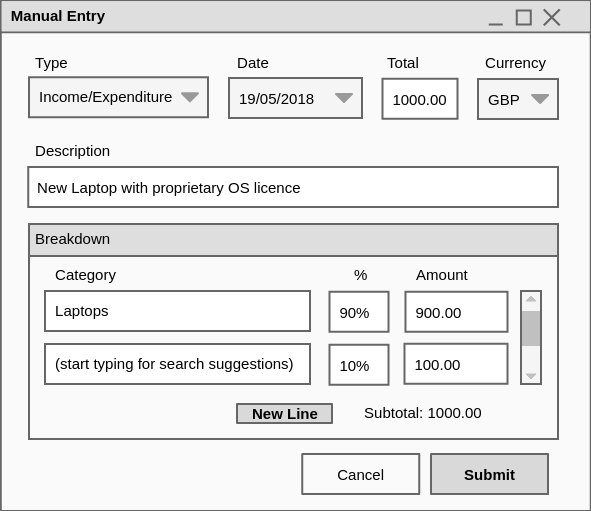
\includegraphics[width=14cm]{./contents/img/Wireframe_-_Manual_Entry.png}
  \end{center}
  \caption{User interface wireframe for \emph{Create Manual Entry} use case}
  \label{fig:Wireframe.CreateManualEntry}
\end{figure}
\FloatBarrier

And in order to better understand the relationship between \emph{Upload
Statement} and \emph{Categorise Entries}, the activity diagram below (Figure
\ref{fig:AD.CategoriseEntries}) was developed:
\begin{figure}[ht!]
  \begin{center}
    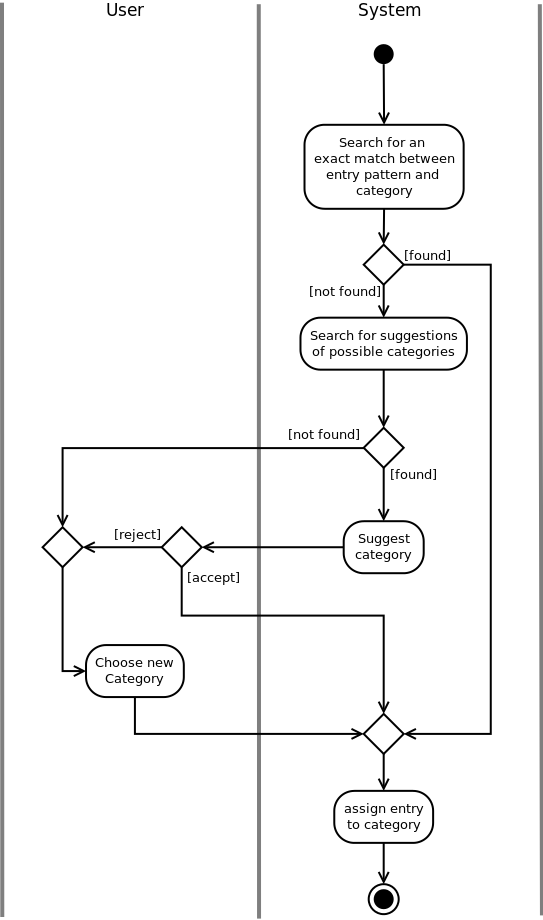
\includegraphics[width=11cm]{./contents/img/Activity_Diagram_-_Categorise_Entries.png}
  \end{center}
  \caption{}
  \label{fig:AD.CategoriseEntries}
\end{figure}
\FloatBarrier


\subsection{Non-Functional Requirements} \label{sec:Requirements.NonFunctionalRequirements}
Use cases and use case diagrams are an appropriate tool to document functional
requirements, but not non-functional ones (Jacobson et al., 1999,
\cite[cited][p.~153]{bennett2010object}). Therefore, a separate list has been
kept in order to document the non-functional requirements, where they exist.
% TODO: make sure I've actually got a list once I understand what these
% requirements are
